\documentclass[12pt,a4paper]{article}

\usepackage[a4paper,margin=1in]{geometry}
\usepackage{graphicx}
\usepackage{booktabs}
\usepackage{amsmath,amssymb}
\usepackage{float}
\usepackage{hyperref}
\usepackage{xcolor}
\usepackage{listings}
\usepackage{enumitem}
\usepackage{fancyhdr}
\usepackage{longtable}
\usepackage{subcaption}   % required for the 2-graphs-per-row layout
\usepackage{mathptmx}     % Times New Roman substitute font (text + math)
\usepackage{fontawesome} % for using icons

\hypersetup{colorlinks=true,linkcolor=blue,urlcolor=blue}

\pagestyle{fancy}
\fancyhf{}
\lhead{ICS1512}
\rhead{Machine Learning Algorithms Laboratory}
\cfoot{\thepage}

\lstset{
language=Python,
basicstyle=\ttfamily\small,
numbers=left,
frame=single,
breaklines=true,
showstringspaces=false
}

\begin{document}

\begin{tabular}{|p{4cm}|p{11cm}|}
\hline
Experiment No. & 3\\ \hline
Experiment Title & Regression Analysis using Linear and Regularized Models \href{https://github.com/Poojashree81/ICS1512-Machine-Learning-Laboratory.git}{\faGithub} \\ \hline
Student Name & Poojashree V \\ \hline
Register Number & 3122247001043 \\ \hline
Faculty & Dr. Poreddy Ajay Kumar Reddy \\ \hline
Submission Date & 21st July 2026\\ \hline
\end{tabular}

\section{Objective}\label{sec:objective}
This experiment implements Linear Regression along with three regularized variants -- Ridge, Lasso, and Elastic Net -- to predict a continuous target (the sanctioned loan amount). We tune regularization strength using 5-fold cross-validated Grid Search, then evaluate all four models on MAE, MSE, RMSE, $R^2$, and training time. Beyond the numbers, we also look at residual and coefficient plots to get a feel for how each model actually behaves, and spend some time digging into overfitting, underfitting, and the bias--variance trade-off across the four.

\section{Problem Statement}\label{sec:problem}
Given a loan applicant's demographic, financial, and property-related attributes (age, income, profession, credit score, requested loan amount, property price, and so on), the task is to predict \textbf{Loan Sanction Amount (USD)} -- a continuous numerical value. This is a supervised \textbf{regression} problem: the input is a mixed-type feature vector (numerical and categorical), and the output is a single real-valued prediction. We're not just chasing the lowest prediction error here -- the bigger question is how L1 and L2 penalties reshape the model's coefficients, affect its generalization gap, and change its variance relative to plain Ordinary Least Squares (OLS).

\section{Dataset Description}\label{sec:dataset}
\begin{longtable}{|p{6cm}|p{8cm}|}
\hline
Dataset Name & Predict Loan Amount Data \\ \hline
Dataset Source & Kaggle -- dataset \textit{phileinsophos/predict-loan-amount-data} \\ \hline
Number of Samples & 29{,}660 (after dropping rows with a missing target; in practice none were dropped, since the target column had zero missing values) \\ \hline
Number of Features & 20 raw features (11 numerical + 9 categorical) once the three identifier columns are dropped (\texttt{Customer ID}, \texttt{Name}, \texttt{Property ID}); this expands to \textbf{53} features after one-hot encoding the categorical columns \\ \hline
Number of Classes & Not applicable -- this is a regression task with a continuous target (\texttt{Loan Sanction Amount (USD)}) \\ \hline
Missing Values & Present in 10 of the 20 feature columns. The biggest gaps are \texttt{Type of Employment} (7{,}188, 24.2\%), \texttt{Property Age} (4{,}760, 16.1\%), \texttt{Income (USD)} (4{,}493, 15.1\%), \texttt{Dependents} (2{,}446, 8.2\%), \texttt{Credit Score} (1{,}670, 5.6\%), \texttt{Income Stability} (1{,}658, 5.6\%), \texttt{Has Active Credit Card} (1{,}546, 5.2\%), \texttt{Property Location} (347, 1.2\%), \texttt{Current Loan Expenses (USD)} (167, 0.6\%), and \texttt{Gender} (52, 0.2\%). The target column itself came through with no missing values at all. \\ \hline
Train-Test Split & 80:20 (23{,}728 training samples / 5{,}932 test samples), \texttt{random\_state=42}; hyperparameters were tuned separately, using 5-fold cross-validation strictly \textit{within} the training split. \\ \hline
\end{longtable}

\section{Exploratory Data Analysis}\label{sec:eda}

\begin{itemize}
\item \textbf{Dataset overview:} 29{,}660 rows $\times$ 24 raw columns (20 usable features + 3 identifier columns + 1 target).
\item \textbf{Statistical summary:} The numeric features live on very different scales -- \texttt{Age} sits in the 18--65 range, \texttt{Income (USD)} runs from a few hundred up past $10^5$, and \texttt{Property Price} climbs into the hundreds of thousands of USD. That gap alone is basically the reason feature scaling is non-negotiable before Ridge/Lasso/Elastic Net (see Section~\ref{sec:algorithm}).
\item \textbf{Missing value analysis:} 10 of 20 feature columns carry missing values, anywhere from 0.2\% (\texttt{Gender}) to 24.2\% (\texttt{Type of Employment}). None of them was missing badly enough to justify dropping the column outright.
\item \textbf{Target distribution:} Right-skewed (Figure~\ref{fig:target_dist}) -- most sanctioned loans cluster toward the lower end, with a long tail of a few unusually large sanctioned amounts.
\item \textbf{Feature vs.\ target relationships:} We looked at \texttt{Age}, \texttt{Income (USD)}, and \texttt{Loan Amount Request (USD)} specifically (Figures~\ref{fig:age_vs_target}--\ref{fig:loanreq_vs_target}).
\item \textbf{Feature distributions:} All 11 numeric and 9 categorical features were plotted individually (Figures~\ref{fig:numeric_dist} and \ref{fig:categorical_dist}).
\item \textbf{Correlation matrix / class distribution:} Not applicable / not generated in this run -- there are no classes in a regression task, and a full numeric correlation heatmap wasn't part of the notebook we actually ran. Worth adding later with \texttt{df.corr()} + \texttt{seaborn.heatmap()} on the numeric subset, if needed.
\end{itemize}

\begin{figure}[H]
\centering
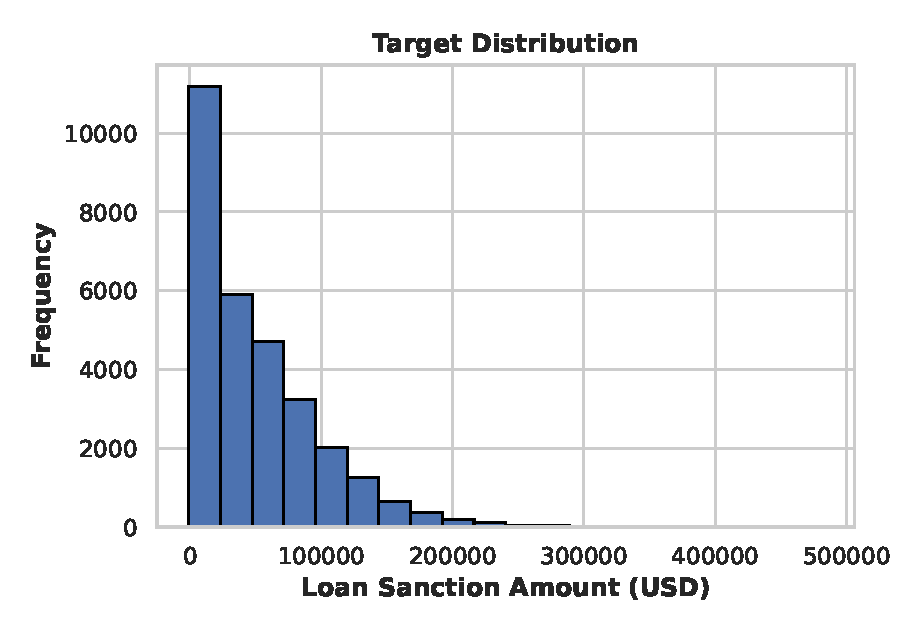
\includegraphics[width=0.6\linewidth]{figures/target_distribution.eps}
\caption{Distribution of the target variable, Loan Sanction Amount (USD)}\label{fig:target_dist}
\end{figure}

\textbf{Inference:} From Figure~\ref{fig:target_dist} we can see the target is strongly right-skewed -- most applicants get relatively modest sanctioned amounts, while a small number receive very large sanctions, stretching the tail out to roughly 3--4$\times$ the modal value. This is probably a big part of why RMSE comes out noticeably larger than MAE for every model in Section~\ref{sec:results}: squared error punishes those few large-loan outliers much more heavily. One thing worth trying in a future pass, though we didn't do it here, is a log-transform of the target.

\begin{figure}[H]
\centering
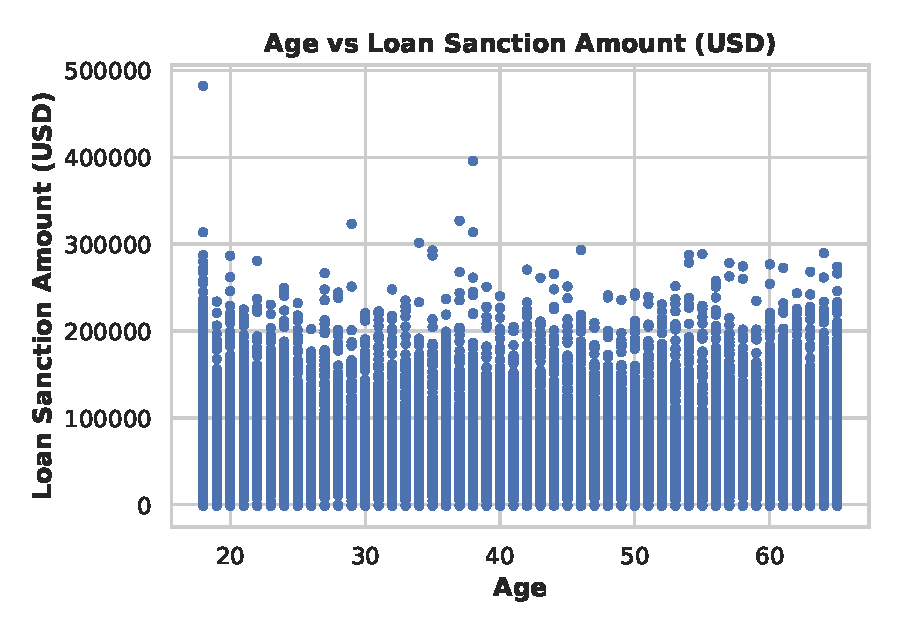
\includegraphics[width=0.55\linewidth]{figures/Age_vs_target.eps}
\caption{Age vs. Loan Sanction Amount (USD)}\label{fig:age_vs_target}
\end{figure}

\textbf{Inference:} The points here are scattered almost uniformly across the whole age range (18--65), for basically every value of the target. There's no obvious upward or downward trend. One possible explanation is that \texttt{Age} alone just doesn't carry much linear predictive signal for the sanctioned amount -- and that lines up with it getting a fairly small coefficient magnitude in the trained models later (see Figure~\ref{fig:coef_comparison}).

\begin{figure}[H]
\centering
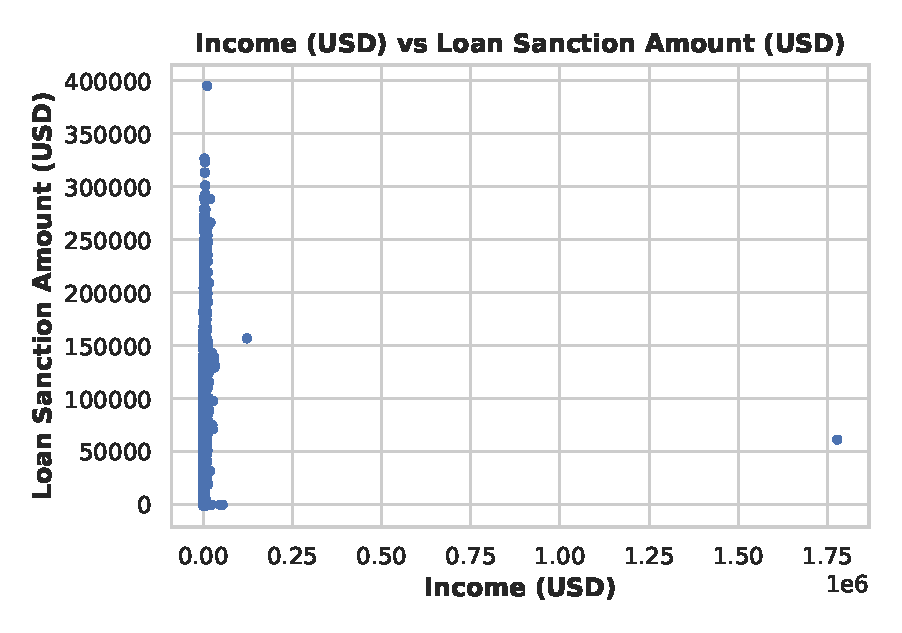
\includegraphics[width=0.55\linewidth]{figures/Income_USD__vs_target.eps}
\caption{Income (USD) vs. Loan Sanction Amount (USD)}\label{fig:income_vs_target}
\end{figure}

\textbf{Inference:} Most applicants earn below 20{,}000 USD, and even inside that dense cluster the sanctioned amount swings widely -- anywhere from close to 0 up to around 300{,}000 USD. A handful of high-income applicants (up to $\sim$180{,}000 USD) don't seem to get proportionally bigger sanctions either. Taken together, this points to income being a fairly noisy, weak predictor once other things like loan request size and credit score are factored in.

\begin{figure}[H]
\centering
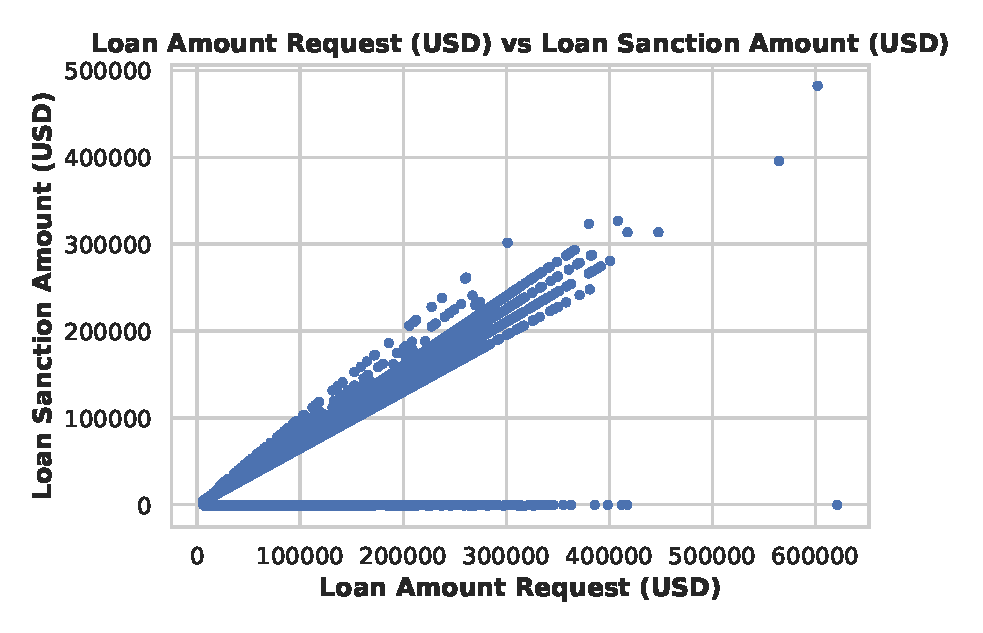
\includegraphics[width=0.55\linewidth]{figures/Loan_Amount_Request_USD__vs_target.eps}
\caption{Loan Amount Request (USD) vs. Loan Sanction Amount (USD)}\label{fig:loanreq_vs_target}
\end{figure}

\textbf{Inference:} This is easily the clearest relationship in the whole EDA -- the points form a tight, roughly linear diagonal band, meaning the sanctioned amount scales almost proportionally with what was requested (banks typically sanction some fraction of the requested sum). We'd expect this single feature to dominate the linear model's predictions, and the coefficient plot in Figure~\ref{fig:coef_comparison} confirms that's exactly what happens.

\subsection*{Numeric Feature Distributions}

\begin{figure}[H]
\centering
\begin{subfigure}{0.31\linewidth}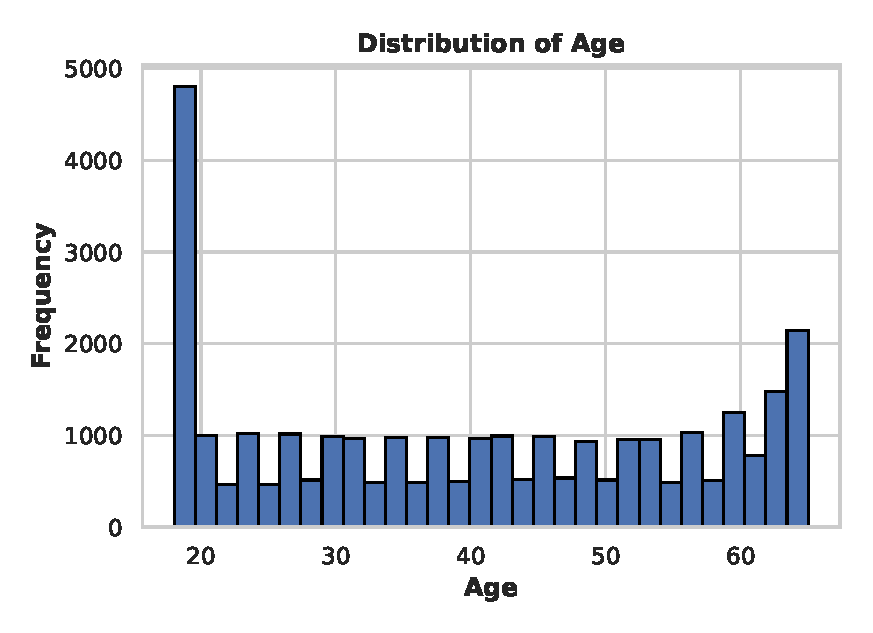
\includegraphics[width=\linewidth]{figures/dist_Age.eps}\caption{Age}\end{subfigure}\hfill
\begin{subfigure}{0.31\linewidth}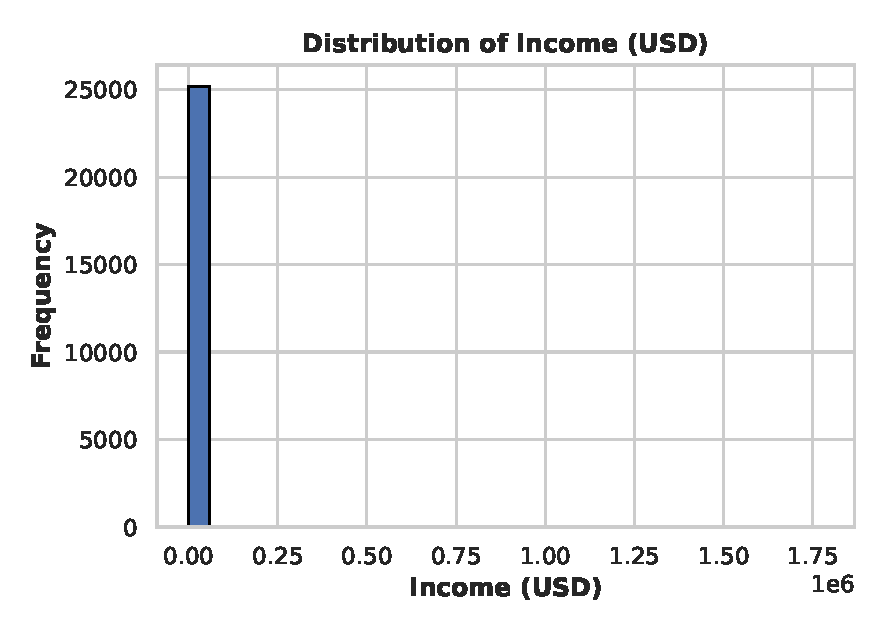
\includegraphics[width=\linewidth]{figures/dist_Income_USD.eps}\caption{Income (USD)}\end{subfigure}\hfill
\begin{subfigure}{0.31\linewidth}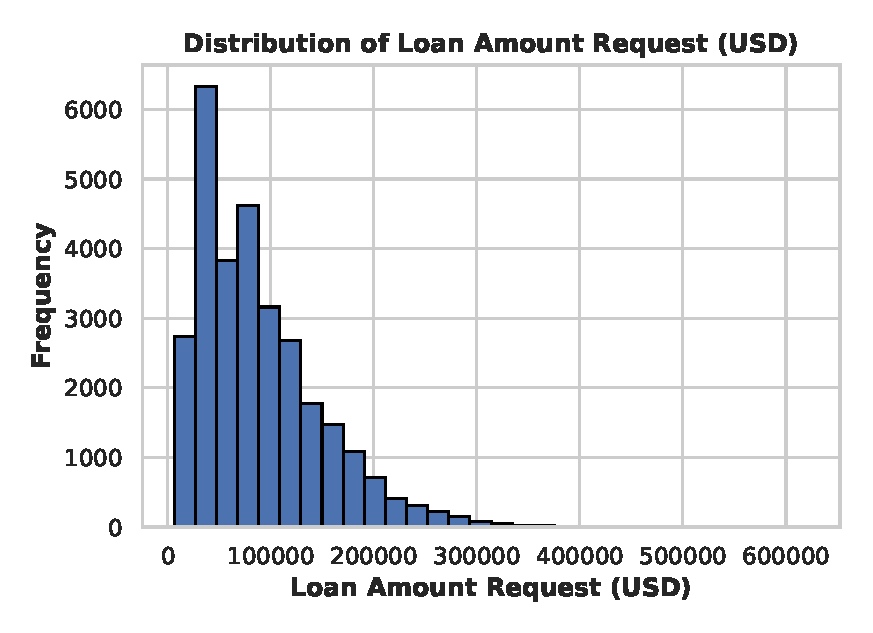
\includegraphics[width=\linewidth]{figures/dist_Loan_Amount_Request_USD.eps}\caption{Loan Amount Request (USD)}\end{subfigure}

\vspace{0.4cm}
\begin{subfigure}{0.31\linewidth}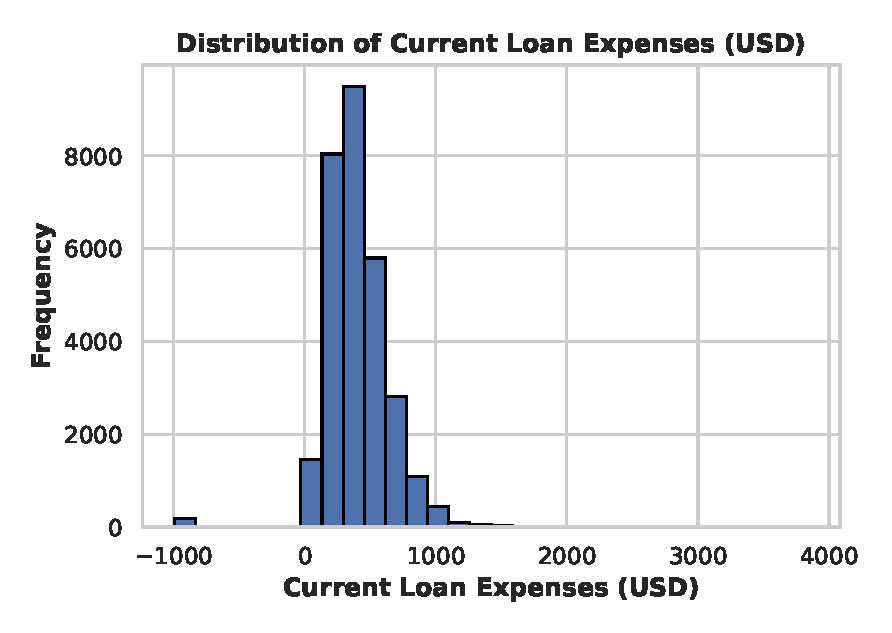
\includegraphics[width=\linewidth]{figures/dist_Current_Loan_Expenses_USD.eps}\caption{Current Loan Expenses (USD)}\end{subfigure}\hfill
\begin{subfigure}{0.31\linewidth}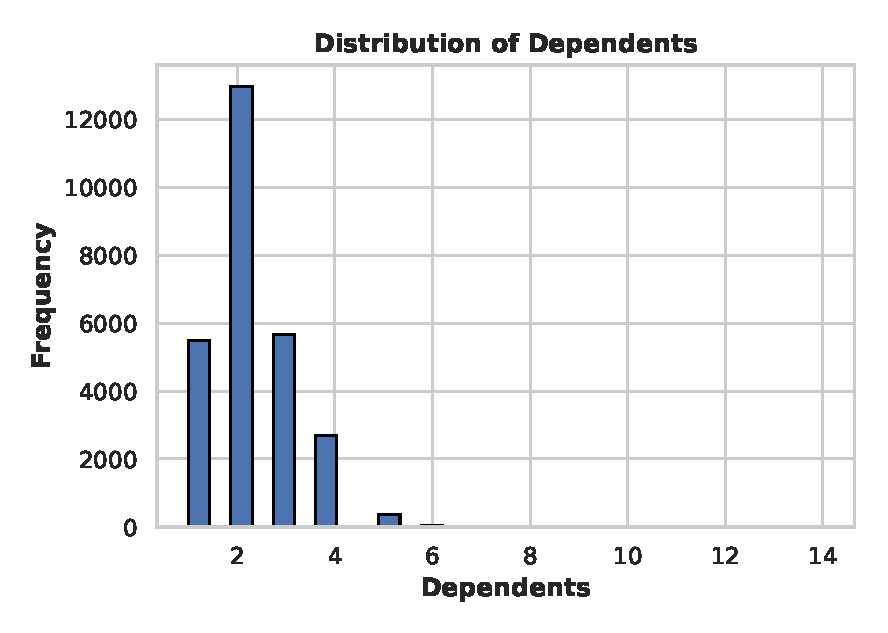
\includegraphics[width=\linewidth]{figures/dist_Dependents.eps}\caption{Dependents}\end{subfigure}\hfill
\begin{subfigure}{0.31\linewidth}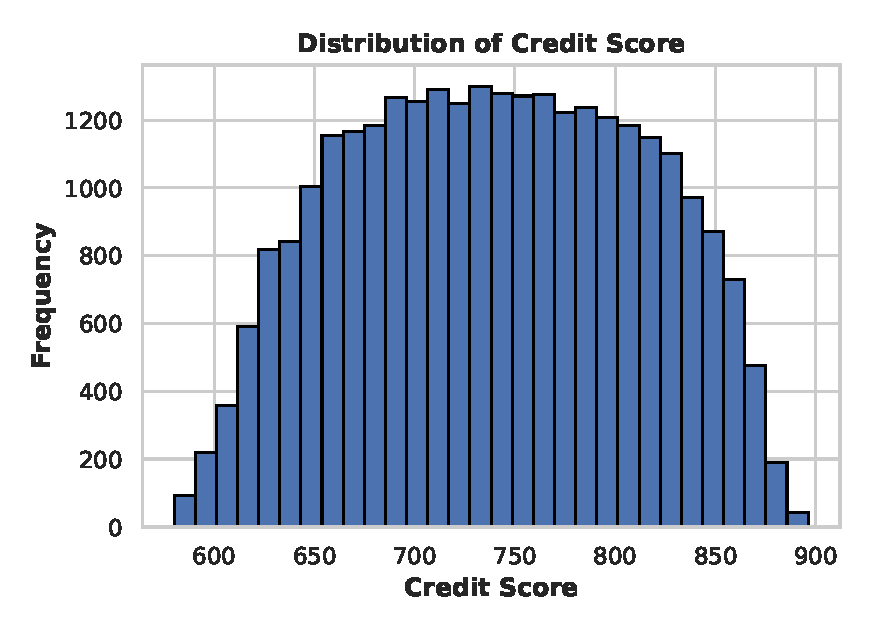
\includegraphics[width=\linewidth]{figures/dist_Credit_Score.eps}\caption{Credit Score}\end{subfigure}

\vspace{0.4cm}
\begin{subfigure}{0.31\linewidth}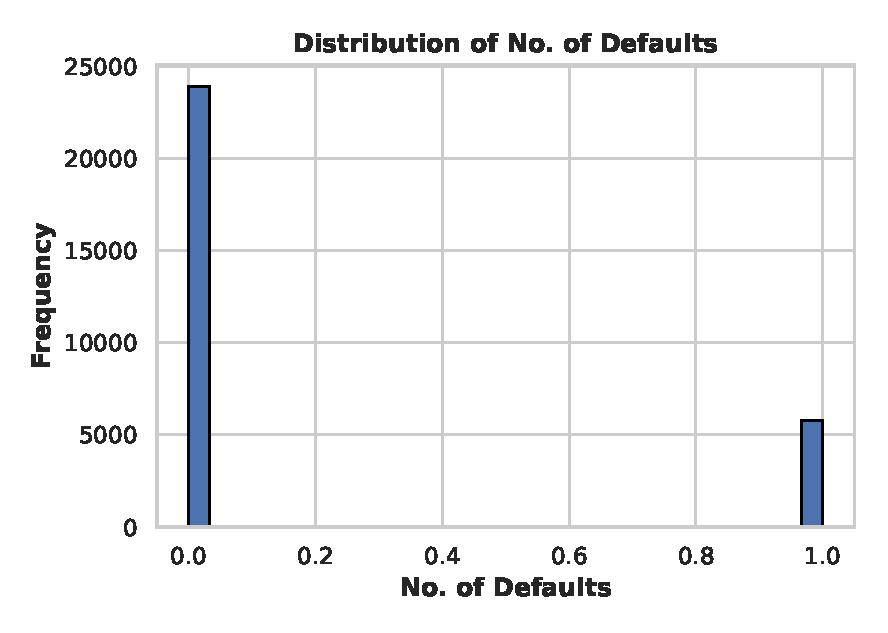
\includegraphics[width=\linewidth]{figures/dist_No_of_Defaults.eps}\caption{No. of Defaults}\end{subfigure}\hfill
\begin{subfigure}{0.31\linewidth}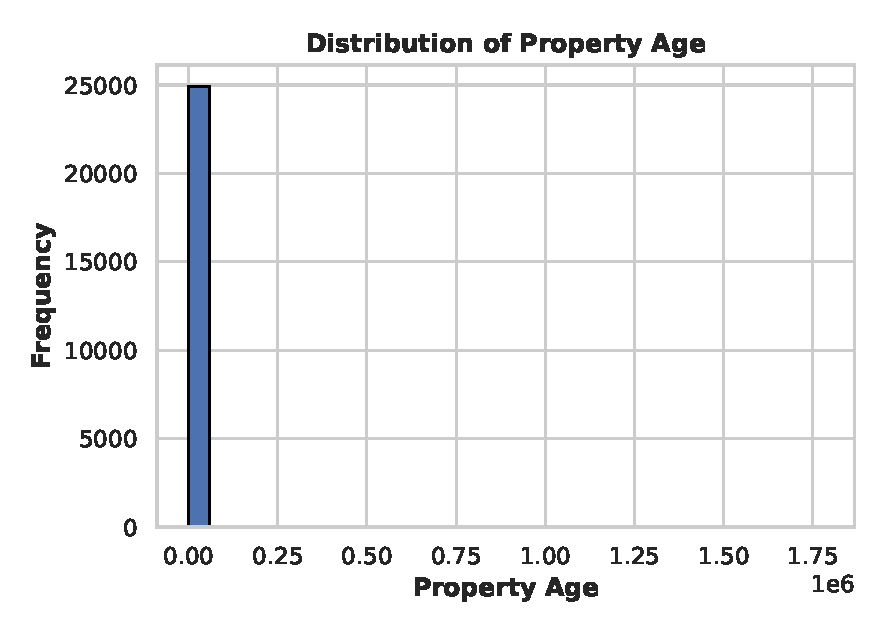
\includegraphics[width=\linewidth]{figures/dist_Property_Age.eps}\caption{Property Age}\end{subfigure}\hfill
\begin{subfigure}{0.31\linewidth}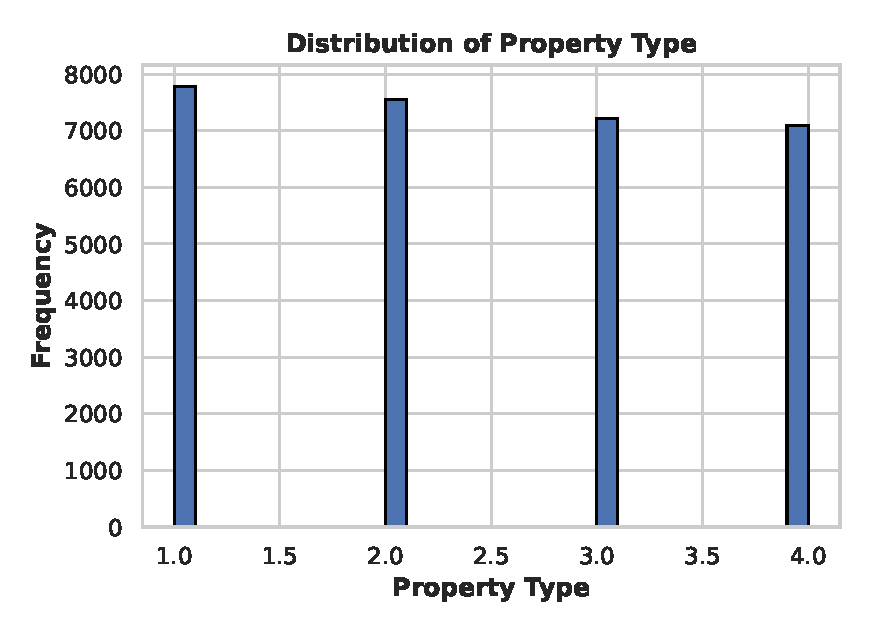
\includegraphics[width=\linewidth]{figures/dist_Property_Type.eps}\caption{Property Type}\end{subfigure}

\vspace{0.4cm}
\begin{subfigure}{0.31\linewidth}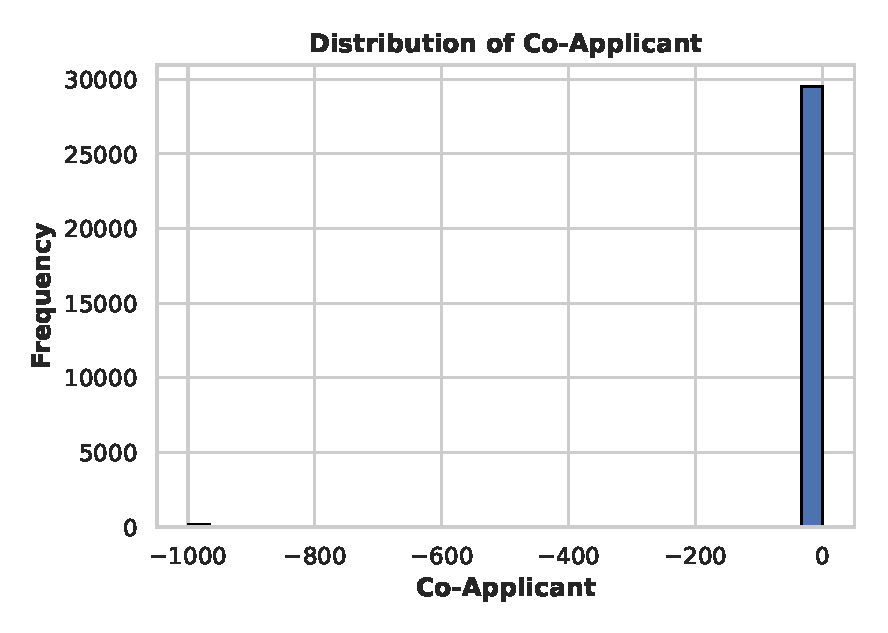
\includegraphics[width=\linewidth]{figures/dist_Co-Applicant.eps}\caption{Co-Applicant}\end{subfigure}\hfill
\begin{subfigure}{0.31\linewidth}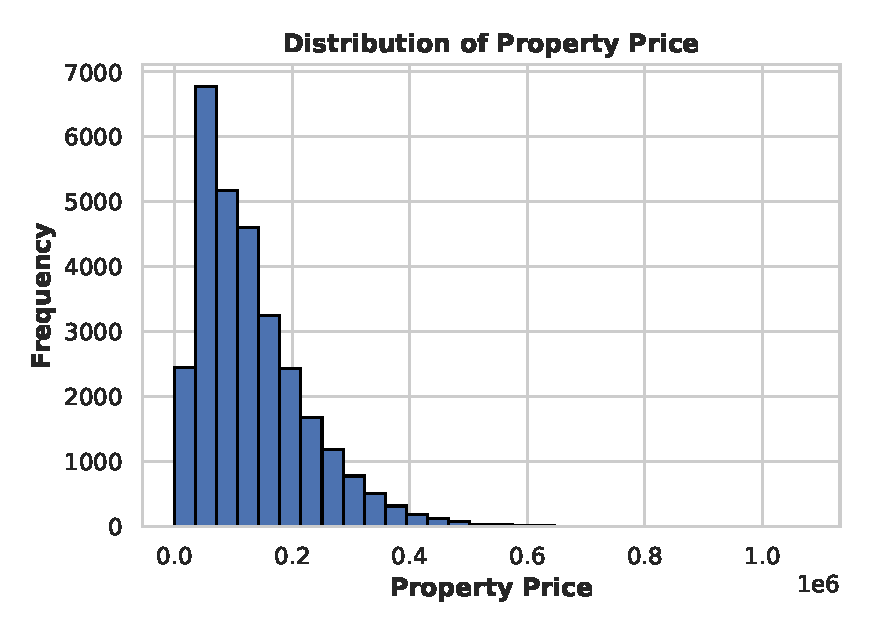
\includegraphics[width=\linewidth]{figures/dist_Property_Price.eps}\caption{Property Price}\end{subfigure}
\caption{Distributions of all 11 numeric features}
\label{fig:numeric_dist}
\end{figure}

\textbf{Inference:} \texttt{Income (USD)}, \texttt{Loan Amount Request (USD)}, and \texttt{Current Loan Expenses (USD)} are all heavily right-skewed with a long tail of high-value outliers, which fits with the extreme income outlier ($\sim$1.78 million USD) we already saw in Figure~\ref{fig:income_vs_target}. \texttt{Age} spreads fairly evenly across its 18--65 range -- no surprise, given the uniform scatter in Figure~\ref{fig:age_vs_target}. \texttt{No. of Defaults}, \texttt{Dependents}, and \texttt{Co-Applicant} are discrete, low-cardinality count features that pile up at small integer values (0, 1, 2), so just a couple of bars dominate each histogram.

\subsection*{Categorical Feature Distributions}

\begin{figure}[H]
\centering
\begin{subfigure}{0.31\linewidth}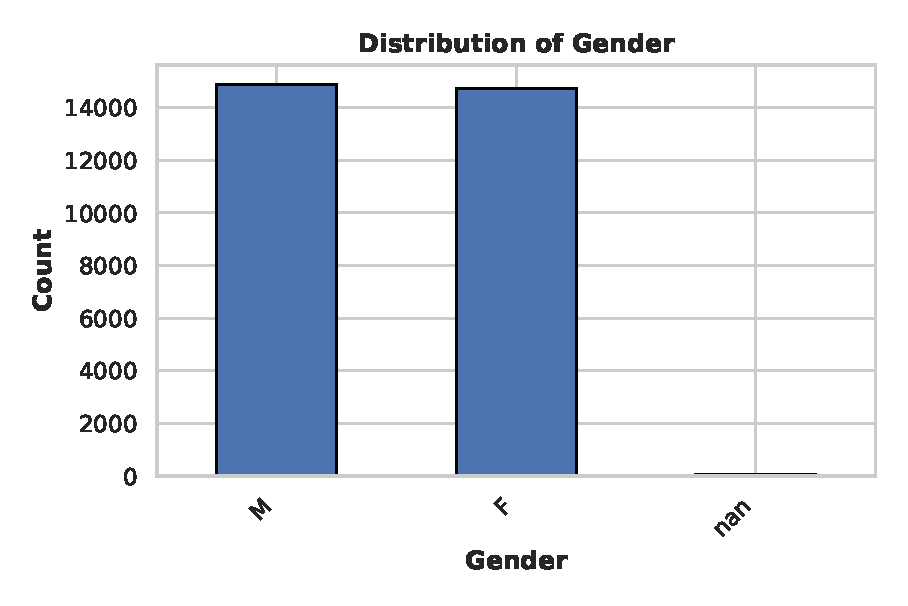
\includegraphics[width=\linewidth]{figures/dist_Gender.eps}\caption{Gender}\end{subfigure}\hfill
\begin{subfigure}{0.31\linewidth}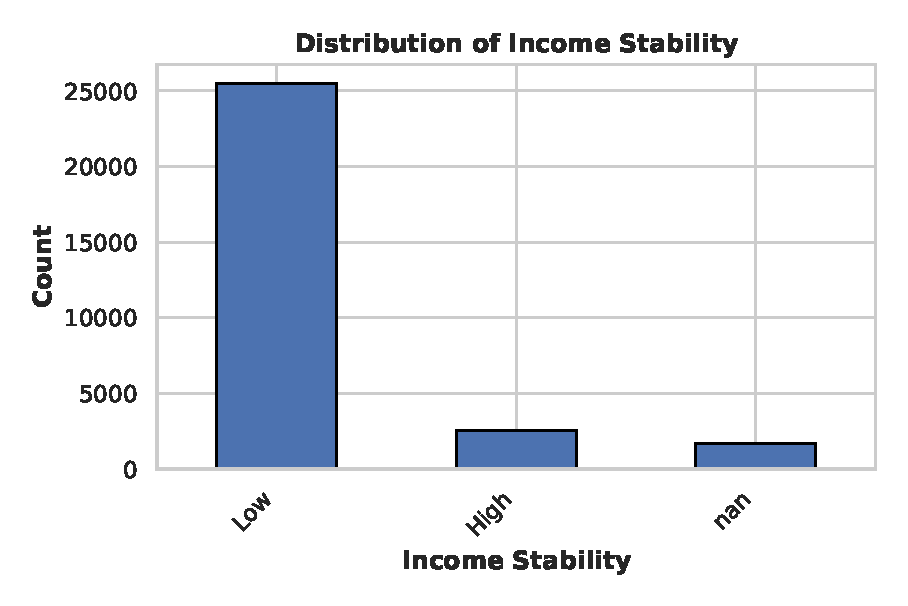
\includegraphics[width=\linewidth]{figures/dist_Income_Stability.eps}\caption{Income Stability}\end{subfigure}\hfill
\begin{subfigure}{0.31\linewidth}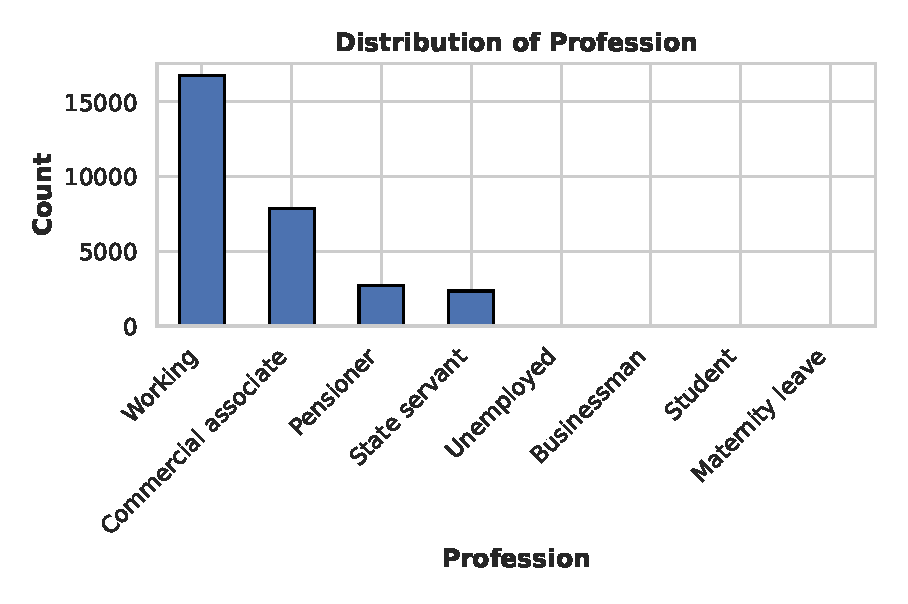
\includegraphics[width=\linewidth]{figures/dist_Profession.eps}\caption{Profession}\end{subfigure}

\vspace{0.4cm}
\begin{subfigure}{0.31\linewidth}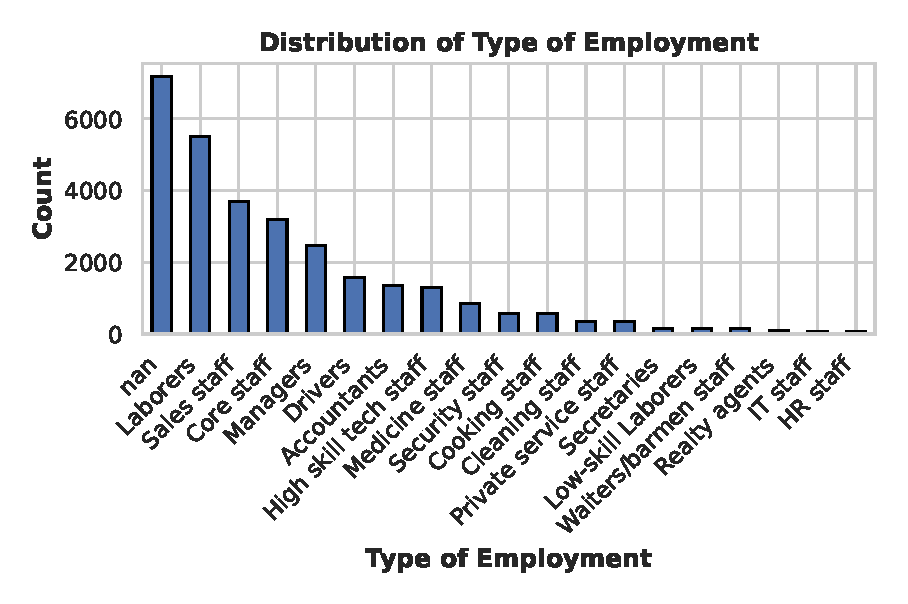
\includegraphics[width=\linewidth]{figures/dist_Type_of_Employment.eps}\caption{Type of Employment}\end{subfigure}\hfill
\begin{subfigure}{0.31\linewidth}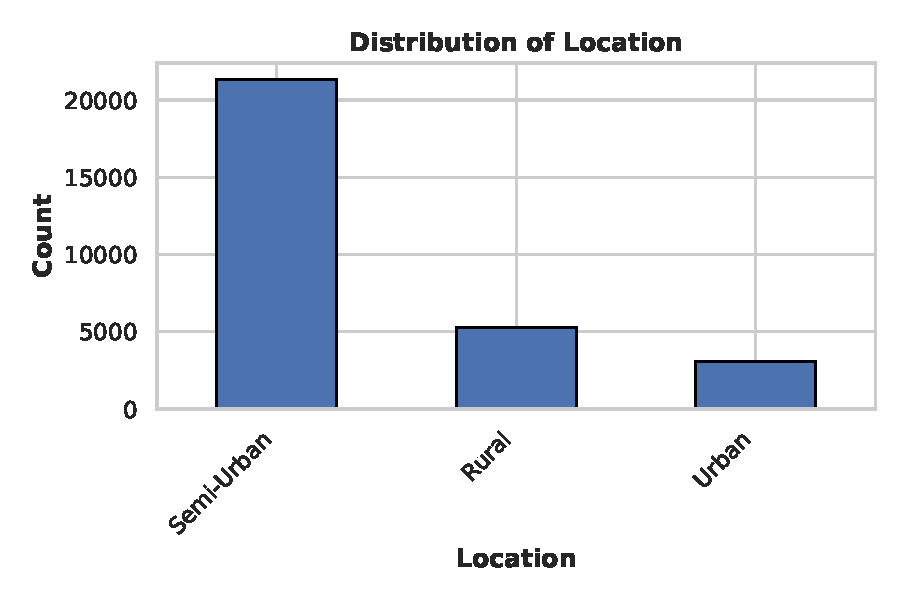
\includegraphics[width=\linewidth]{figures/dist_Location.eps}\caption{Location}\end{subfigure}\hfill
\begin{subfigure}{0.31\linewidth}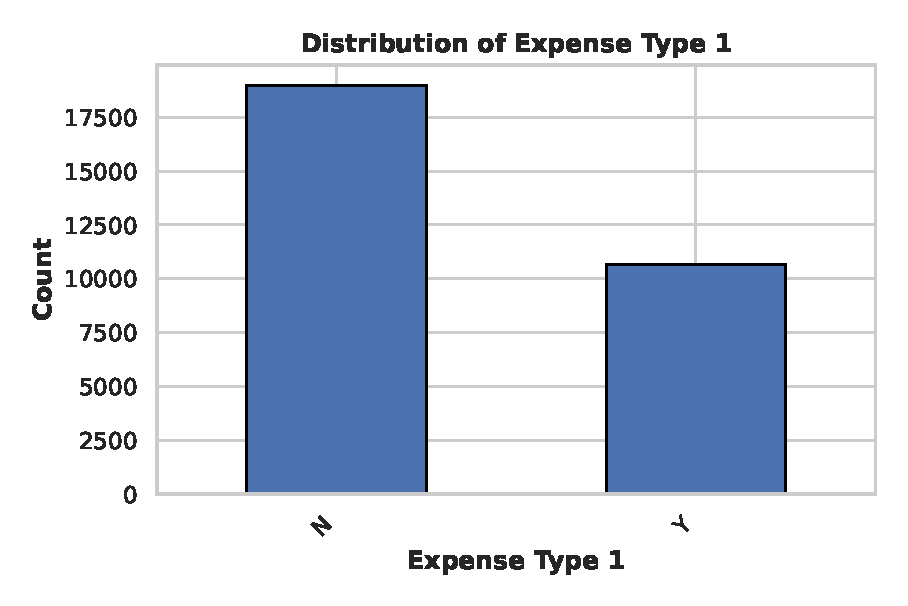
\includegraphics[width=\linewidth]{figures/dist_Expense_Type_1.eps}\caption{Expense Type 1}\end{subfigure}

\vspace{0.4cm}
\begin{subfigure}{0.31\linewidth}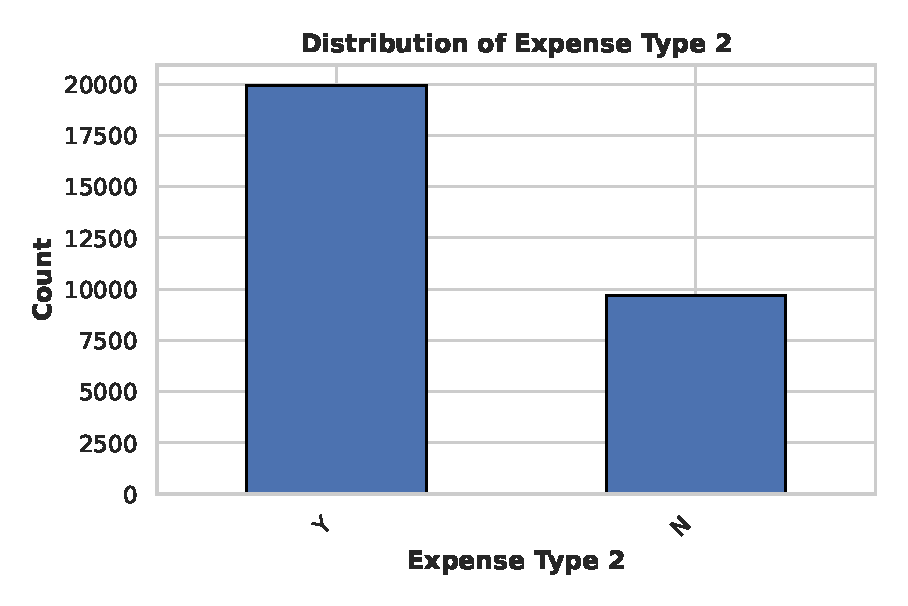
\includegraphics[width=\linewidth]{figures/dist_Expense_Type_2.eps}\caption{Expense Type 2}\end{subfigure}\hfill
\begin{subfigure}{0.31\linewidth}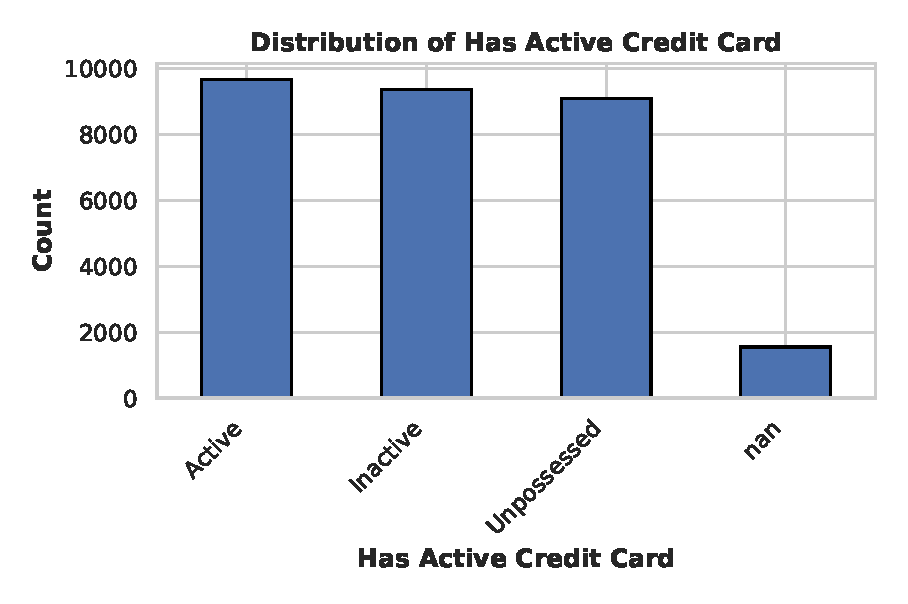
\includegraphics[width=\linewidth]{figures/dist_Has_Active_Credit_Card.eps}\caption{Has Active Credit Card}\end{subfigure}\hfill
\begin{subfigure}{0.31\linewidth}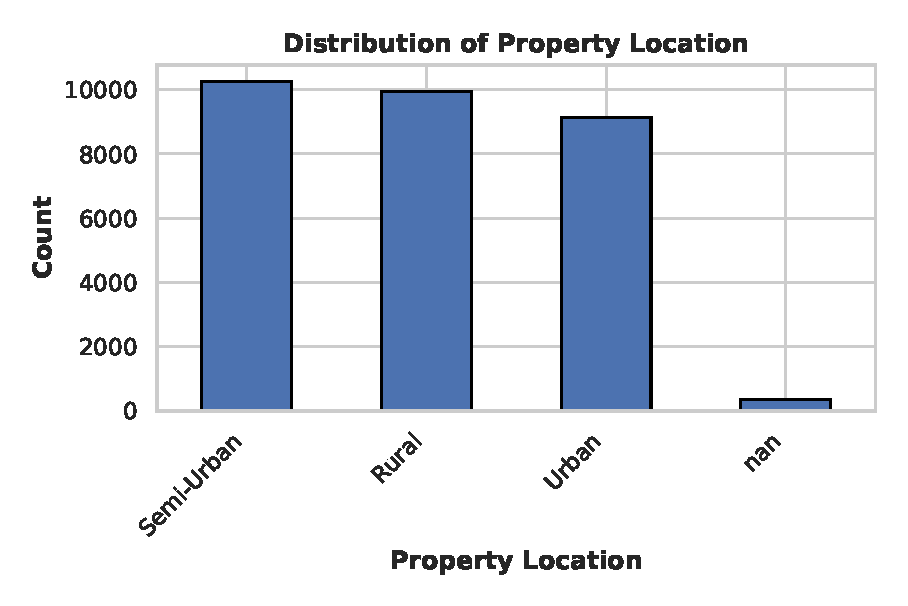
\includegraphics[width=\linewidth]{figures/dist_Property_Location.eps}\caption{Property Location}\end{subfigure}
\caption{Distributions of all 9 categorical features (bar height = category count, including a bar for missing/NaN where present)}
\label{fig:categorical_dist}
\end{figure}

\textbf{Inference:} These bar charts show the raw category counts for each categorical column, and they include missing values as their own bar -- consistent with the null counts back in Section~\ref{sec:dataset}, so for instance \texttt{Type of Employment} shows a clearly visible NaN bar reflecting its 24.2\% missing rate. We're leaving the exact per-category proportions to the charts themselves rather than restating every number here, since \texttt{value\_counts()} output wasn't printed alongside the plots in the notebook we ran.

\section{Data Preprocessing}\label{sec:preprocessing}

\begin{itemize}
\item \textbf{ID removal:} \texttt{Customer ID}, \texttt{Name}, and \texttt{Property ID} were dropped before modeling. They're unique identifiers with zero predictive value, and leaving them in would just leak row identity into the one-hot encoder.
\item \textbf{Missing value handling:} Numeric features were imputed with the \textbf{median} (which holds up well against the outliers we saw in Section~\ref{sec:eda}, e.g.\ in \texttt{Income} and \texttt{Property Price}); categorical features got the \textbf{mode} (most frequent category). Both imputers were fit \textit{only} on the training fold at every stage -- see the next point -- so there's no leakage of test-set statistics into training.
\item \textbf{Encoding:} Categorical columns (\texttt{Gender}, \texttt{Income Stability}, \texttt{Profession}, \texttt{Type of Employment}, \texttt{Location}, \texttt{Expense Type 1}, \texttt{Expense Type 2}, \texttt{Has Active Credit Card}, \texttt{Property Location}) were run through \texttt{OneHotEncoder} (\texttt{handle\_unknown="ignore"}), which is where those 9 categorical columns turn into part of the final 53-column design matrix.
\item \textbf{Feature scaling:} Numeric features were standardized with \texttt{StandardScaler} (zero mean, unit variance). This one's not really optional for this experiment -- Ridge and Lasso penalize the \textit{raw magnitude} of coefficients, so an unscaled feature like \texttt{Property Price} (scale $\sim10^5$) would get punished far more harshly than \texttt{Age} (scale $\sim10^1$) purely because of units, not because it's actually more important.
\item \textbf{Train-test split:} 80:20 split (\texttt{random\_state=42}), done \textbf{before} any preprocessing was fit. All imputation/encoding/scaling steps were wrapped inside a single \texttt{sklearn.pipeline.Pipeline} along with the regressor, so during 5-fold cross-validation each fold's preprocessing statistics (median, mode, mean/std) were computed only on that fold's own training portion -- a leakage-free setup, as far as we can tell.
\item \textbf{Feature engineering:} None beyond what's above -- all 20 raw columns were used as they came.
\end{itemize}

\section{Machine Learning Algorithm}\label{sec:algorithm}

We implemented four related linear models. All of them fit a linear predictor $\hat{y} = \mathbf{w}^\top \mathbf{x} + b$, and the only real difference between them is what penalty (if any) gets added to the ordinary least-squares loss.

\subsection*{Linear Regression (baseline / OLS)}
\textbf{Working principle:} Finds the hyperplane that minimizes the sum of squared residuals between predicted and actual values.
\textbf{Mathematical formulation:}
\[
\min_{\mathbf{w}, b} \; \sum_{i=1}^{n} \left(y_i - \mathbf{w}^\top \mathbf{x}_i - b\right)^2
\]
with the closed-form (normal equation) solution $\mathbf{w} = (X^\top X)^{-1} X^\top y$.
\textbf{Advantages:} Simple, interpretable, no hyperparameters to worry about, and quick to train (0.24 s here).
\textbf{Limitations:} Nothing stops coefficient magnitude from growing; it's unstable when features are correlated (multicollinearity), and it's prone to overfitting once the number of one-hot encoded features gets large relative to the actual signal -- which is somewhat the case here, with 53 features.

\subsection*{Ridge Regression (L2 regularization)}
\textbf{Working principle:} Adds a penalty proportional to the \textit{squared} magnitude of the coefficients, which shrinks all of them smoothly toward zero without ever forcing any to exactly zero.
\textbf{Mathematical formulation:}
\[
\min_{\mathbf{w}, b} \; \sum_{i=1}^{n} \left(y_i - \mathbf{w}^\top \mathbf{x}_i - b\right)^2 + \alpha \sum_{j} w_j^2
\]
with closed-form solution $\mathbf{w} = (X^\top X + \alpha I)^{-1} X^\top y$.
\textbf{Advantages:} Cuts down variance/instability from correlated features; still has a closed-form solution, so it trains quickly even with a 5-value grid search (4.9 s here).
\textbf{Limitations:} It never actually performs feature selection -- all 53 coefficients stay non-zero -- and the single $\alpha$ shrinks every coefficient by a comparable relative amount, regardless of how important any given one actually is.

\subsection*{Lasso Regression (L1 regularization)}
\textbf{Working principle:} Adds a penalty proportional to the \textit{absolute} magnitude of the coefficients. Because the L1 penalty has a sharp corner at zero, it can drive individual coefficients all the way to exactly zero, which amounts to automatic feature selection.
\textbf{Mathematical formulation:}
\[
\min_{\mathbf{w}, b} \; \sum_{i=1}^{n} \left(y_i - \mathbf{w}^\top \mathbf{x}_i - b\right)^2 + \alpha \sum_{j} |w_j|
\]
There's no closed-form solution here; it's solved iteratively via coordinate descent.
\textbf{Advantages:} Produces sparse, more interpretable models -- in this experiment it zeroed out 16 of 53 coefficients (30.2\% sparsity) at its selected $\alpha$.
\textbf{Limitations:} Coordinate descent has to converge iteratively, which is a lot slower than Ridge's closed form (44.3 s here -- the slowest of all four models). With correlated features it also tends to arbitrarily pick one from a correlated group and zero out the rest, which can make it unstable across resamples. Worth flagging: several small-$\alpha$ candidates in this experiment's grid search actually triggered \texttt{ConvergenceWarning}s (duality gap around $10^{12}$ against \texttt{max\_iter=3000}), meaning the optimizer hadn't fully converged for those candidates -- we come back to this caveat in Section~\ref{sec:discussion}.

\subsection*{Elastic Net (combined L1 + L2 regularization)}
\textbf{Working principle:} Linearly blends the Ridge and Lasso penalties, controlled by a mixing parameter \texttt{l1\_ratio} $\in [0,1]$ (1 = pure Lasso, 0 = pure Ridge).
\textbf{Mathematical formulation:}
\[
\min_{\mathbf{w}, b} \; \sum_{i=1}^{n} \left(y_i - \mathbf{w}^\top \mathbf{x}_i - b\right)^2 + \alpha \left(\rho \sum_j |w_j| + \frac{1-\rho}{2} \sum_j w_j^2\right), \quad \rho = \texttt{l1\_ratio}
\]
\textbf{Advantages:} Gets Ridge's stability on correlated features \textit{and} a bit of Lasso's sparsity. In practice, it came out with the best validation $R^2$ of all four models here (0.5797).
\textbf{Limitations:} Two hyperparameters ($\alpha$ and \texttt{l1\_ratio}) instead of one means a bigger search space (12 combinations here) and slower training (25.1 s). At the selected \texttt{l1\_ratio}=0.2, it didn't actually zero out any coefficients in this run (0.0\% sparsity) -- so it ended up behaving more like Ridge than Lasso.

\section{Experimental Setup}
\begin{tabular}{ll}
\toprule
Python Version & 3.12 \\
Scikit-Learn Version & 1.6.1 \\
IDE & Jupyter Notebook \\
Operating System & Linux (Ubuntu-based) \\
Hardware & CPU \\
\bottomrule
\end{tabular}

\section{Hyperparameter Selection}\label{sec:hyperparam}

\subsection*{Table 1 -- Hyperparameter Tuning Summary}
\begin{longtable}{|p{3.2cm}|p{2.6cm}|p{5.5cm}|p{2.3cm}|}
\hline
\textbf{Model} & \textbf{Search Method} & \textbf{Best Parameters} & \textbf{Best CV $R^2$} \\ \hline
Ridge Regression & Grid Search & $\alpha = 100$ (searched over $\{0.01, 0.1, 1, 10, 100\}$) & 0.5689 \\ \hline
Lasso Regression & Grid Search & $\alpha = 10$ (searched over $\{0.001, 0.01, 0.1, 1, 10\}$) & 0.5685 \\ \hline
Elastic Net Regression & Grid Search & $\alpha = 0.1$, \texttt{l1\_ratio} $= 0.2$ (searched over $\alpha \in \{0.01,0.1,1,10\}$, \texttt{l1\_ratio} $\in \{0.2,0.5,0.8\}$) & 0.5736 \\ \hline
\end{longtable}

Worth flagging here: in all three cases the search pushed toward one edge of the grid we specified (Ridge and Lasso both landed on their \textit{largest} tested $\alpha$). That's a signal the true optimum might sit outside the tested range, so extending the grid further -- say up to $\alpha=1000$ -- would be a sensible next step, rather than treating 100/10 as confirmed optima.

\section{Results}\label{sec:results}

\subsection*{Table 2 -- Cross-Validation Performance (5-Fold, on training set)}
{\small
\begin{tabular}{lcccc}
\toprule
Model & MAE & MSE & RMSE & $R^2$ \\
\midrule
Linear Regression & 21{,}508.85 & $9.848 \times 10^{8}$ & 31{,}381.40 & 0.5779 \\
Ridge Regression & 21{,}525.52 & $9.831 \times 10^{8}$ & 31{,}354.21 & 0.5786 \\
Lasso Regression & 21{,}498.39 & $9.835 \times 10^{8}$ & 31{,}360.41 & 0.5784 \\
Elastic Net Regression & 21{,}842.81 & $9.814 \times 10^{8}$ & 31{,}326.87 & \textbf{0.5797} \\
\bottomrule
\end{tabular}
}

\subsection*{Table 3 -- Test Set Performance}
{\small
\begin{tabular}{lccccc}
\toprule
Model & MAE & MSE & RMSE & $R^2$ & Training Time (s) \\
\midrule
Linear Regression & 21{,}589.12 & $1.0189 \times 10^{9}$ & 31{,}920.75 & 0.5511 & \textbf{0.243} \\
Ridge Regression & 21{,}581.58 & $1.0173 \times 10^{9}$ & 31{,}894.37 & \textbf{0.5518} & 4.942 \\
Lasso Regression & 21{,}564.13 & $1.0178 \times 10^{9}$ & 31{,}902.45 & 0.5516 & 44.302 \\
Elastic Net Regression & 21{,}850.24 & $1.0213 \times 10^{9}$ & 31{,}957.76 & 0.5500 & 25.136 \\
\bottomrule
\end{tabular}
}

\vspace{0.3cm}
\textbf{Best model on the held-out test set: Ridge Regression} ($R^2 = 0.5518$), and only by a thin margin over Lasso and plain Linear Regression. What's interesting is that Elastic Net had the \textit{best} cross-validation $R^2$ (0.5797) but ends up the \textit{worst} on the test set (0.5500) -- a good reminder that whatever ranking CV gives you doesn't always carry over cleanly to the untouched test set, especially when the models are this close together (all four sit within $\sim$0.003 $R^2$ of each other on test).

\subsection*{Table 4 -- Effect of Regularization on Coefficients}
We're leaving the exact coefficient values to Figure~\ref{fig:coef_comparison} (Section~\ref{sec:visualization}) rather than typing them out as raw numbers here, since reading precise values off a bar chart isn't really reliable anyway. The qualitative pattern for the ten features with the largest $|{\rm Linear}|$ coefficient looks like this:

\begin{longtable}{|p{4.3cm}|p{2cm}|p{7cm}|}
\hline
\textbf{Feature} & \textbf{Sign} & \textbf{Observation across Linear $\to$ Ridge $\to$ Lasso $\to$ Elastic Net} \\ \hline
Loan Amount Request (USD) & Positive & By far the largest-magnitude coefficient of any feature in the model -- visibly taller than every other bar in Figure~\ref{fig:coef_comparison}, which tracks with the strong linear trend we saw back in Figure~\ref{fig:loanreq_vs_target}. \\ \hline
Credit Score & Positive & Second-largest positive driver; its magnitude shrinks moderately under Ridge/Lasso/Elastic Net. \\ \hline
Property Price & Positive & Stays consistently positive; sees moderate shrinkage across the regularized models. \\ \hline
Type of Employment = Unemployed & Negative & A large negative coefficient under plain Linear Regression that visibly shrinks toward zero moving to Ridge $\to$ Lasso $\to$ Elastic Net -- probably the clearest example of shrinkage anywhere in the plot. \\ \hline
Has Active Credit Card = Unpossessed & Negative & A moderate negative effect that shrinks under regularization. \\ \hline
Current Loan Expenses (USD), Expense Type 2 = Y & Negative & Small-to-moderate negative coefficients, shrunk further by regularization. \\ \hline
Profession = Working, Property Age, Income Stability = Low & Mixed, near zero & The smallest-magnitude coefficients among the top 10; they contribute little no matter which model you look at. \\ \hline
\end{longtable}

\section{Result Visualization}\label{sec:visualization}

\begin{figure}[H]
\centering
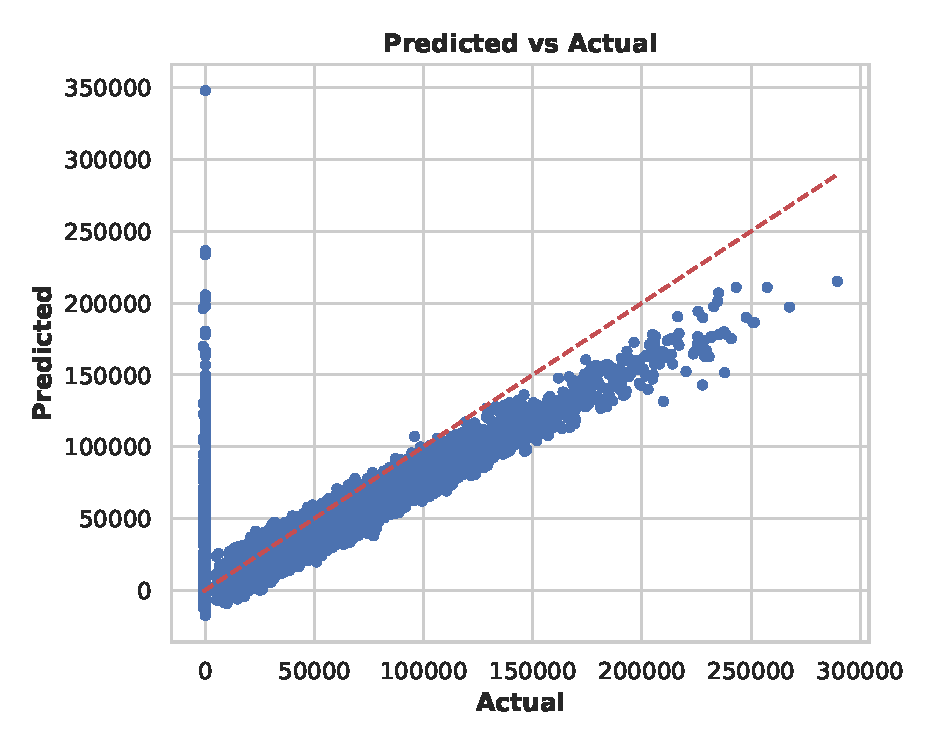
\includegraphics[width=0.55\linewidth]{figures/predicted_vs_actual.eps}
\caption{Predicted vs. Actual Loan Sanction Amount -- best model (Ridge Regression)}\label{fig:pred_actual}
\end{figure}

\textbf{Inference:} Looking at Figure~\ref{fig:pred_actual}, predictions track the ideal $y=x$ line (red dashed) fairly well for small-to-mid sanctioned amounts, but the model clearly under-predicts at the high end -- actual values above roughly 150{,}000 USD keep coming out lower than they should, almost like the predictions "cap out" there. This is probably the clearest visual explanation for why $R^2$ tops out around 0.55: the model captures most of the trend but systematically compresses the right (high-value) tail of that skewed target distribution we saw back in Figure~\ref{fig:target_dist}.

\begin{figure}[H]
\centering
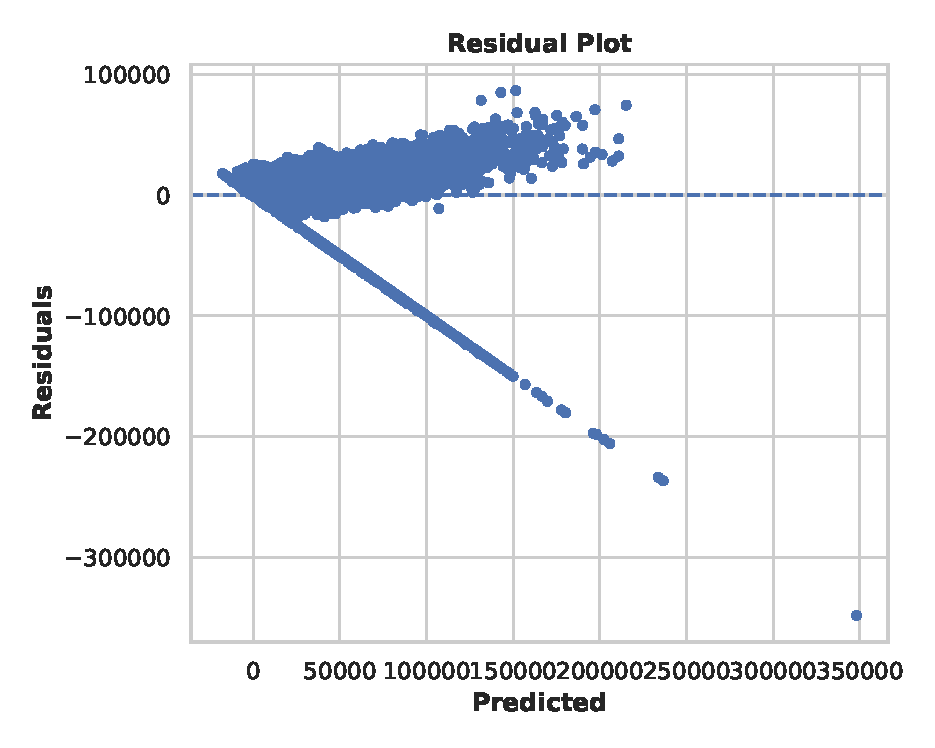
\includegraphics[width=0.55\linewidth]{figures/residual_plot.eps}
\caption{Residual plot -- best model (Ridge Regression)}\label{fig:residual}
\end{figure}

\textbf{Inference:} From Figure~\ref{fig:residual} we can see the residuals fan out as the predicted value gets larger -- a fairly classic heteroscedasticity pattern. In plain terms, the model's errors aren't uniformly sized across the prediction range; large predicted loans carry much bigger absolute errors than small ones do. That's technically a violation of the constant-variance assumption behind OLS-style linear models. One possible explanation is that a target transform (like $\log$) or a model that can represent changing variance (gradient boosting, say) might reduce this pattern in future work.

\begin{figure}[H]
\centering
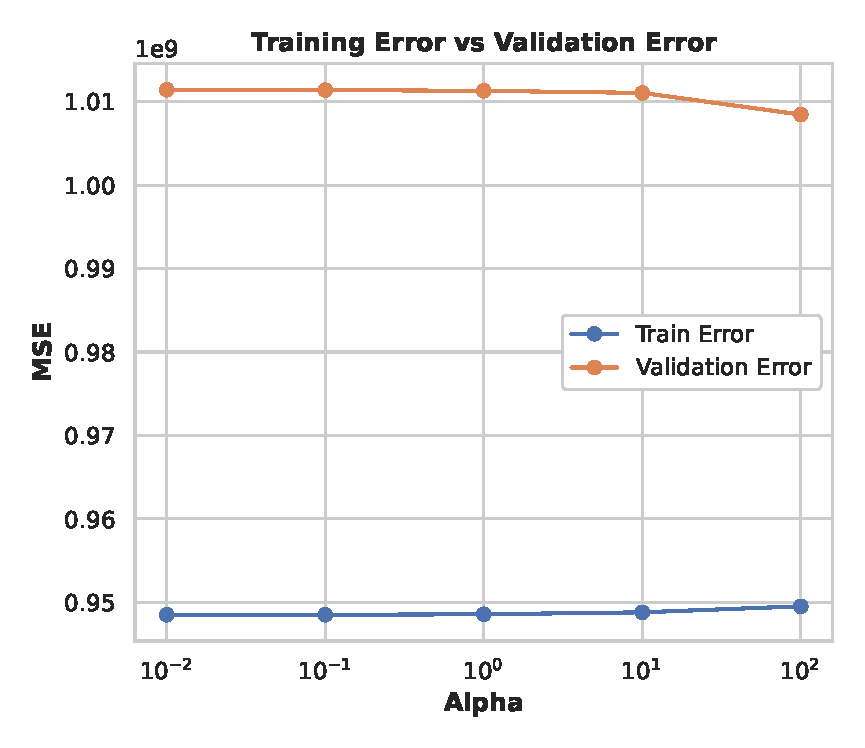
\includegraphics[width=0.55\linewidth]{figures/training_vs_validation_error.eps}
\caption{Training error vs. Validation error across Ridge $\alpha$ (log scale)}\label{fig:train_val}
\end{figure}

\textbf{Inference:} Training and validation MSE start off close together at low $\alpha$ (near plain OLS) and pretty much stay that way as $\alpha$ increases, with validation error edging down slightly and converging toward the training curve near $\alpha=100$ -- the value Grid Search ultimately picked. This fits with the small train/validation $R^2$ gap we report in Section~\ref{sec:discussion} (0.0153 for Ridge): this dataset only shows mild overfitting to begin with, so regularization here is more about fine-tuning than rescuing a badly overfit model.

\begin{figure}[H]
\centering
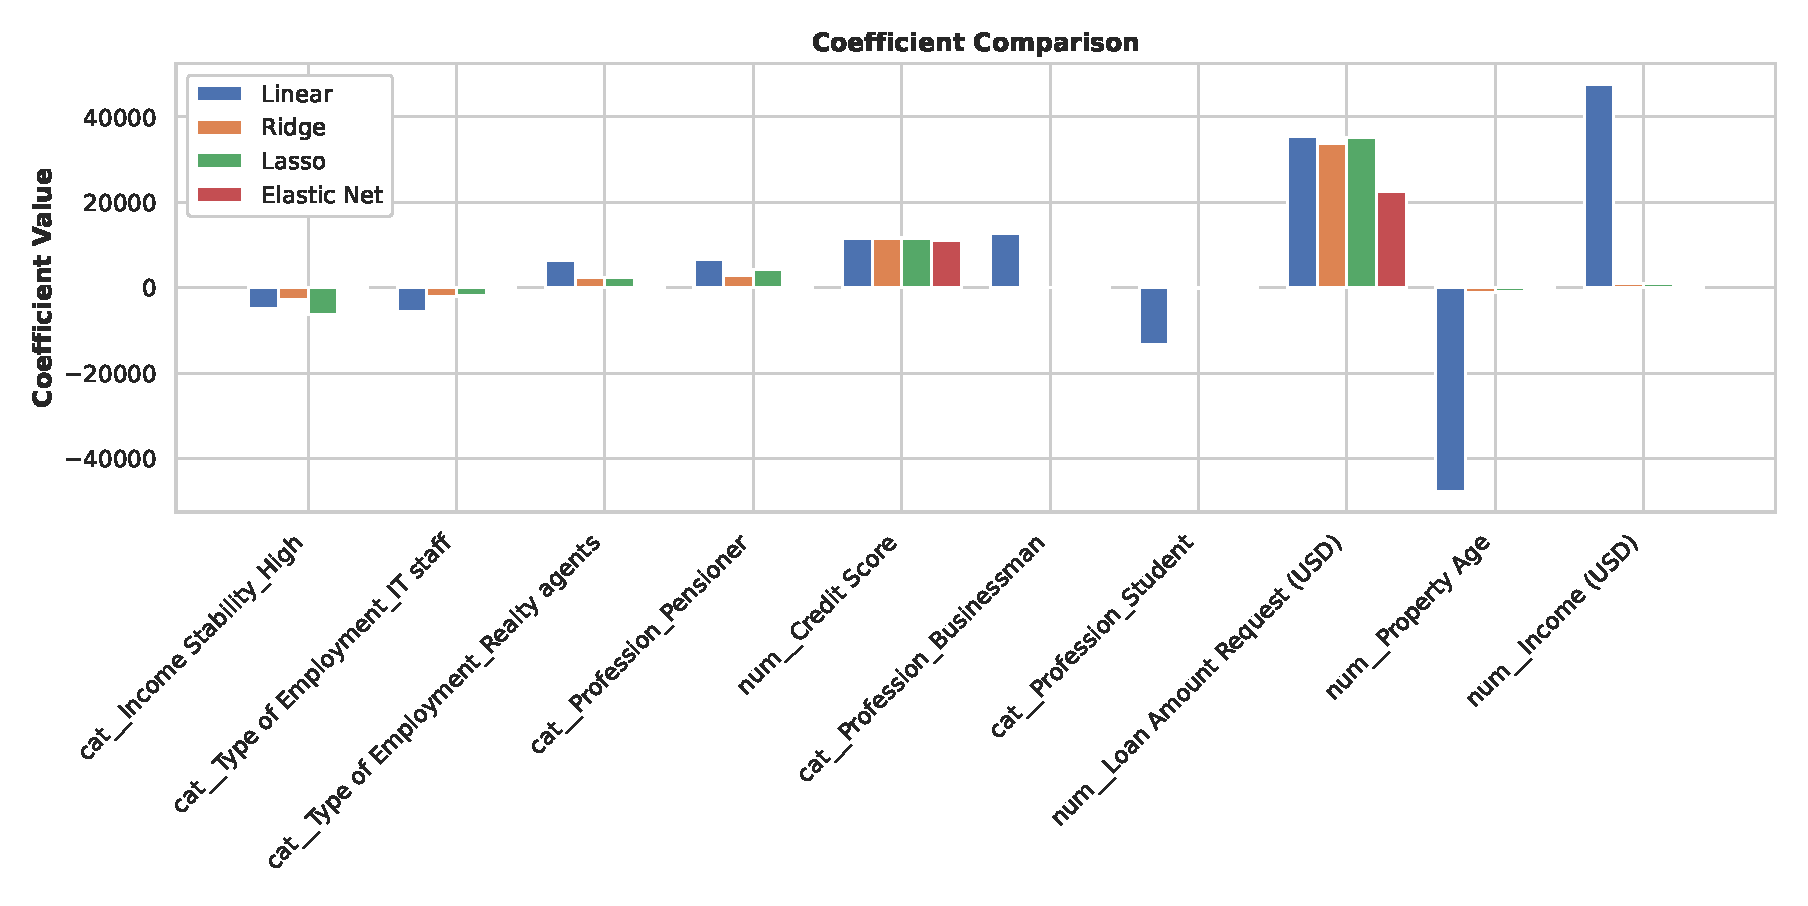
\includegraphics[width=0.75\linewidth]{figures/coefficient_comparison.eps}
\caption{Coefficient comparison across Linear, Ridge, Lasso, and Elastic Net (top 10 features by $|{\rm Linear\ coefficient}|$)}\label{fig:coef_comparison}
\end{figure}

\textbf{Inference:} \texttt{Loan Amount Request (USD)} dominates every model's coefficient vector here, which confirms it as the single most important predictor by a wide margin. Moving left-to-right across each feature group (Linear $\to$ Ridge $\to$ Lasso $\to$ Elastic Net), the bars generally shrink toward zero -- most noticeably for \texttt{Type of Employment = Unemployed}, which is about as clean a visual confirmation as you'll get that all three regularization schemes are doing exactly what they're mathematically designed to do: shrink coefficient magnitude and cut down variance.

\section{Discussion}\label{sec:discussion}

\subsection*{Overfitting and Underfitting Analysis}
We computed the gap between training and validation $R^2$ for all four models (5-fold CV, on the training split):

\begin{center}
\begin{tabular}{lccc}
\toprule
Model & Train $R^2$ & Val $R^2$ & Gap \\
\midrule
Linear Regression & 0.5943 & 0.5779 & 0.0165 \\
Ridge Regression & 0.5939 & 0.5786 & 0.0153 \\
Lasso Regression & 0.5941 & 0.5784 & 0.0156 \\
Elastic Net Regression & 0.5866 & 0.5797 & \textbf{0.0070} \\
\bottomrule
\end{tabular}
\end{center}

All four gaps are pretty small -- well under the conventional 0.05 threshold that's typically used as a rule of thumb for "noticeable overfitting" -- so none of the four models is overfitting badly. This isn't a high-variance regime. Elastic Net has the smallest train/validation gap (0.0070), which makes sense given it's the most heavily regularized of the four (combined L1+L2 penalty). At the same time, none of the models gets anywhere close to explaining the majority of the variance (Train $R^2 \approx 0.59$ across the board), so there's a real \textbf{underfitting} story here too: a purely linear function of these 53 features just can't capture everything going on with the sanctioned-amount target. Cranking up regularization strength (higher $\alpha$) only narrowed the train/validation gap marginally -- Ridge's validation $R^2$ improved by just $+0.0008$ over plain Linear Regression, Lasso by $+0.0006$, Elastic Net by $+0.0018$ -- which tells us regularization isn't really the bottleneck here; the linear model form itself is.

\subsection*{Bias--Variance Analysis}
As a rough proxy for coefficient variance/instability, we computed the standard deviation of the fitted coefficients for each model:

\begin{center}
\begin{tabular}{lc}
\toprule
Model & Coefficient Std. Dev. \\
\midrule
Linear Regression & 11{,}147.68 \\
Ridge Regression & 5{,}023.78 \\
Lasso Regression & 5{,}250.50 \\
Elastic Net Regression & \textbf{3{,}629.72} \\
\bottomrule
\end{tabular}
\end{center}

Plain Linear Regression has by far the widest coefficient spread (11{,}147.68), which fits with it being the lowest-bias / highest-variance model of the four -- it fits the training data most freely and is most easily thrown off by noise and correlated features. Ridge cuts this spread by more than half (down to 5{,}023.78), which is a pretty direct demonstration of its variance-reduction mechanism (uniform L2 shrinkage). Elastic Net comes out lowest of all (3{,}629.72), which makes sense given it combines Ridge's shrinkage with Lasso's sparsity. On sparsity specifically: Lasso zeroed out 16 of 53 coefficients (30.2\%), doing genuine automatic feature selection, while Elastic Net at its chosen \texttt{l1\_ratio}=0.2 zeroed out none at all (0.0\%) -- at this particular hyperparameter combination it ended up behaving much closer to Ridge than to Lasso in terms of sparsity, even though it had the lowest coefficient variance of the bunch. That's a slightly counterintuitive finding worth calling out on its own: \textit{low variance and sparsity aren't the same thing}, and here Elastic Net got the former without the latter.

\subsection*{Methodological Caveats}
Two things are worth being upfront about rather than glossing over:
\begin{enumerate}
\item \textbf{Lasso convergence:} A number of candidates in Lasso's grid search triggered \texttt{ConvergenceWarning}s from the coordinate-descent solver (duality gaps on the order of $10^{12}$ against a tolerance of roughly $4\times10^{10}$, with \texttt{max\_iter=3000}). The selected $\alpha=10$ probably converged more cleanly than the smaller-$\alpha$ candidates did, but this really should be re-run with a higher \texttt{max\_iter} (say 10{,}000) or a tighter \texttt{tol} just to confirm the reported metrics weren't affected by incomplete optimization.
\item \textbf{Edge-of-grid hyperparameters:} As we noted in Section~\ref{sec:hyperparam}, both Ridge ($\alpha=100$) and Lasso ($\alpha=10$) landed on the \textit{largest} value in their search grid. That's a signal the grid may have been too narrow to begin with, and the true optimal $\alpha$ could well sit beyond what we tested.
\end{enumerate}

\section{Conclusion}\label{sec:conclusion}
All four linear models end up at essentially the same test-set performance ($R^2 \approx 0.55$, RMSE $\approx 31{,}900$--$32{,}000$ USD), with Ridge Regression narrowly ahead on the held-out test set ($R^2=0.5518$) and Elastic Net narrowly ahead on cross-validation ($R^2=0.5797$). The fact that all four are this close suggests that, for this dataset, \textbf{regularization strength isn't really the limiting factor} -- overfitting was already mild for plain Linear Regression (train/validation gap of just 0.0165), so L1/L2 penalties didn't have much headroom left to improve generalization ($\leq 0.0018$ $R^2$ improvement in every case). Where regularization \textit{did} clearly help was in cutting coefficient variance (Linear's coefficient std of 11{,}147.68 nearly cut in half by Ridge, and reduced even further by Elastic Net) and, for Lasso specifically, automatic feature selection (30.2\% sparsity). Given the practical trade-offs at play -- Ridge gets the best test $R^2$ at a fraction of Lasso's training cost (4.9 s vs.\ 44.3 s) -- \textbf{Ridge Regression is the model we'd recommend} for this task if only one has to be deployed, though Elastic Net stays an attractive alternative if some feature sparsity alongside low coefficient variance is what you want. The bigger takeaway here is architectural rather than about hyperparameters: since $R^2 \approx 0.55$--0.58 seems to be the ceiling for \textit{any} linear combination of these 53 features, actually pushing performance further would probably need a model that can capture non-linear interactions -- gradient-boosted trees or a shallow neural network, for instance -- rather than more tuning of $\alpha$.

\section{References}\label{sec:references}
\begin{enumerate}[label={[\arabic*]}]
\item Kaggle, ``Predict Loan Amount Data,'' [Online]. Available: \url{https://www.kaggle.com/datasets/phileinsophos/predict-loan-amount-data}
\item scikit-learn developers, ``Linear Models,'' scikit-learn documentation. [Online]. Available: \url{https://scikit-learn.org/stable/modules/linear_model.html}
\item scikit-learn developers, ``Tuning the hyper-parameters of an estimator,'' scikit-learn documentation. [Online]. Available: \url{https://scikit-learn.org/stable/modules/grid_search.html}
\item A. E. Hoerl and R. W. Kennard, ``Ridge Regression: Biased Estimation for Nonorthogonal Problems,'' \textit{Technometrics}, vol. 12, no. 1, pp. 55--67, 1970.
\item R. Tibshirani, ``Regression Shrinkage and Selection via the Lasso,'' \textit{Journal of the Royal Statistical Society: Series B}, vol. 58, no. 1, pp. 267--288, 1996.
\item H. Zou and T. Hastie, ``Regularization and Variable Selection via the Elastic Net,'' \textit{Journal of the Royal Statistical Society: Series B}, vol. 67, no. 2, pp. 301--320, 2005.
\end{enumerate}

\end{document}